%======================================================================
\chapter{Literature Review}
%======================================================================
\section{Introduction}
Thermo-mechanical simulation of the multi-crystalline Si wafer fabrication process via directionally solidified MGS ingots is a complex problem due to the large number of process parameters involved and the complex properties of silicon. To perform such a task, sufficient knowledge is required of the mechanical properties of silicon, the directional solidification process, the wire sawing process, and finite element modelling. In this chapter, prior literature on these topics is reviewed. The literature can be divided into three distinct areas: (i) constitutive behaviour of Si, (ii) analytical and numerical studies of the directional solidification process, and (iii) analytical and numerical studies of the wire sawing process. 

Experimental studies can be very informative in studying the evolution of dislocations and residual stresses during thermo-mechanical processing. However, experiments involving directional solidification and wire sawing processes require considerable time and costs, so computational models have been developed to simulate the stress and the temperature fields under various cooling rates and material geometries. These models were developed using numerical techniques such as finite element methods and require the mathematical equations behind the the physical processes. The validity of these models, however, needs to be tested against some experimental data. These models can be very helpful to an industrial practitioners who wishes to improve the quality of the products.

\section{Silicon: Properties}
\subsection{Crystal structure and phases}
Si is a covalently bonded material that exists as diamond cubic structure with a face-centered Bravais lattice and a two atom basis. Its lattice parameter is approximately found to be a~0.543 nm at 293 K \cite{hull1999properties}. Si displays allotropy, existing in different phases with a different lattice structures depending on the temperature and pressure. Thermo-mechanical processing of Si leads to phase transformation due to changes in temperature and pressure. This transformation may change the material from ductile to brittle thereby causing failure while during�� processing. At room temperature and 1 bar pressure, Si exists as diamond cubic form Si-I. Indentations and cracks can lead to high stress concentrations and hydrostatic stresses, which can lead to its phase transformation.  Kailer \textit{et al} \cite{kailer1997phase} showed that the cubic Si-I transforms to metallic Si-II at a depth of 0.5 microns under a diamond indenter. This then transforms into amorphous Si at fast unloading rates or a mix of Si-III and Si-XII at slow unloading rates. The area away from the indenter has lower stresses and thus forms Si-IV, which undergoes plastic deformation using the classical dislocation glide and twinning mechanism. Zhang \cite{zhang2004plasticity} has reviewed the different modes of plastic behaviour for surfaces. These modes are summarized in Fig. \ref{fig:phase_trans}. Si undergoes a multi-phase reversible or irreversible transformation depending upon the level of both hydrostatic and deviatoric stresses and loading-unloading conditions. 

\noindent
\begin{minipage}[c]{\textwidth}
\centering
        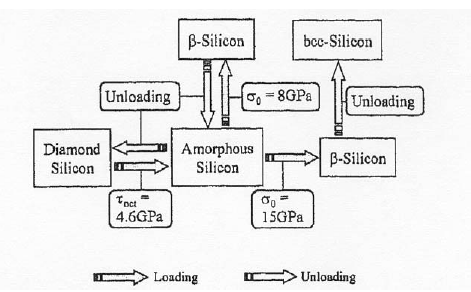
\includegraphics[width=3.0in]{phase-trans.png}
        \captionof{figure}{Phase transformation on Si under stress}
        \label{fig:phase_trans}
 \end{minipage}

\noindent
\begin{minipage}[c]{\textwidth}
\centering
        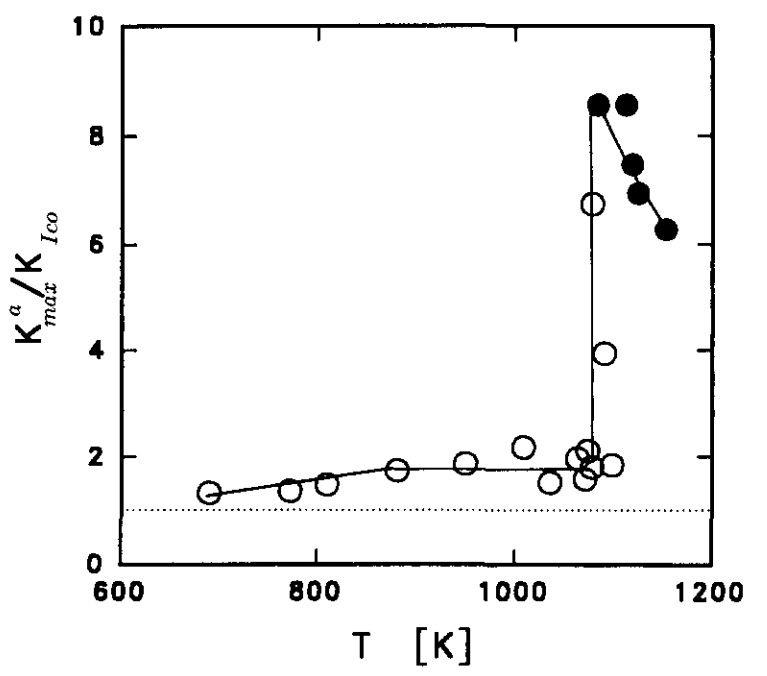
\includegraphics[width=3.0in]{BDT.PNG}
        \captionof{figure}{Brtile to ductile transition of diamond silicon}
        \label{fig:bdt}
 \end{minipage}

Diamond Si has a very high ductile to brittle transition temperature (DBTT); it is brittle at temperatures from ambient to approx. 1000\degree C \cite{brede1993brittle}. It has, however, been also observed that silicon exhibits a ductile behaviour even while processing in brittle regime \cite{liu2007mechanism} under high compressive and sheer stress.
\newline

\subsection{Stress Strain Behaviour}
%\subsubsection{Stress-Strain Behaviour}
Deformation tests have been done \cite{patel1963macroscopic,alexander1969dislocations} to understand the plastic deformation of silicon and germanium crystal at various temperatures and strain rates. These crystals are Float-zone grown and impurity free. These tests are done to understand the different stages of stress-strain curve of silicon. A typically observbed stress-strain curve of a single crystal germanium is shown in Figure \ref{fig:stress-strain}. In the first stage, single crystal exhibits a bell shape stress-strain curve when the strain is less than 2\% of resolved shear strain \cite{patel1963macroscopic}. After stage I, it undergoes two hardening stages, II \& IV and two dynamic recovery stages, III \& V. The inflection in the curve differentiates the various stages.
\noindent
\begin{minipage}[c]{\textwidth}
\centering
       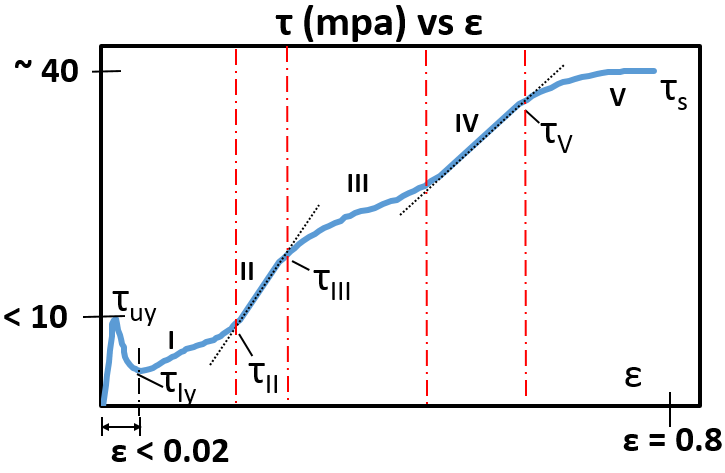
\includegraphics[width=4.0in]{silicon_stress_strain_curve2.PNG}
      \captionof{figure}{Stress-strain curves of germanium monocrystals deformed in tension at different crystallographic orientations at T = 788K and strain rate $\dot{\epsilon} = 2 \times 10^{-3}s^{-1}$}.
        \label{fig:stress-strain}
\end{minipage}

After solidification, the crystal undergoes stage I deformation in which the initial elastic deformation increases the flow stress rapidly till it reaches upper yield stress (UYS), followed by which there is a sharp drop of the flow stress until it reaches the lower yield stress to gradually rise again. The UYS and LYS is dependent on temperature, strain rate and initial dislocation density affect the UYS and the LYS \cite{alexander1969dislocations, yonenaga1978dislocation} as shown:
\begin{equation}
   \tau_{yp} = C_{yp} \dot{\gamma}^{\frac{1}{n_{yp}}} e^{\frac{U_{yp}}{K_{b}T}}
   \label{yield_change}
\end{equation}

Where $C_{yp}$ is a constant with respect to temperature and strain rate, nyp and Uyp are yield point specific parameters and found to be in between 0.45 and 0.8 Tm temperature range [Alexander 1968].
\[U_{uyp} = 1.1, n_{uyp} = 2.1\]
\[U_{lyp} = 0.8, n_{lyp} = 2.9\] 

The variation of UYS with temperature is shown in Figure \ref{fig:stress-temp}. At room temperature the UYS is very high compared to at higher temperature. 

\noindent
\begin{minipage}[c]{\textwidth}
\centering
       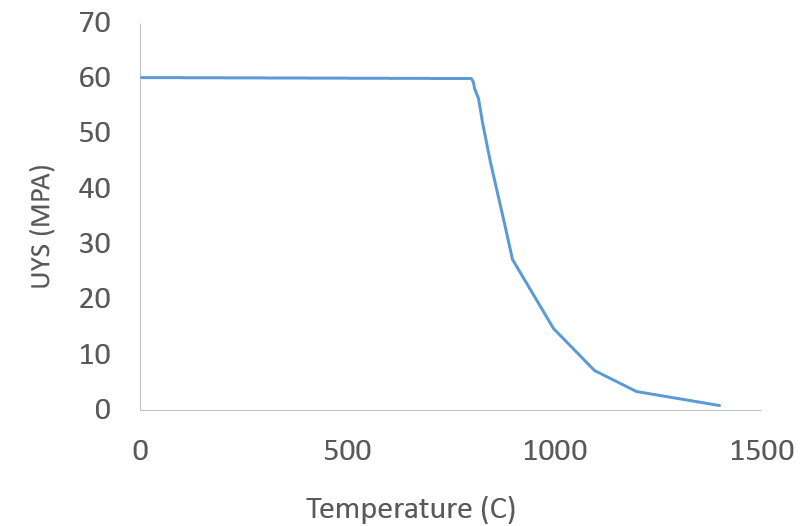
\includegraphics[width=4.0in]{silicon_stress_temp_curve2.PNG}
      \captionof{figure}{Flow stress vs. temperature in silicon for a strain rate of $1.2\times10^{−4} s^{−1}$  \cite{siethoff2001deformation}}.
        \label{fig:stress-temp}
\end{minipage}

\subsection{Dislocation plasticity}

The yield drop is to be due to rapid multiplication of dislocations at UYS. The movement and multiplication of dislocation or dislocation kinetics affects the constitutive behavior of silicon in stage I and so has been reviewed by several researchers the most common of which is given by Alexander-Haasen-Sumino equation written as:
\begin{equation}
   \frac{d\rho_{m}}{dt} = K \rho_{m} v\label{has_1}
\end{equation}
where, $K$ is a function characterizing the dislocation multiplication rate, $v$ is the velocity of the dislocations and $\rho_{m}$ is the change in dislocation density.

A dislocation plasticity constitutive behavior of a material can be used to calculate the dislocation growth and residual stress during application of load while the thermo-mechanical processing. In any such process, the total strain under application of stress can be split into elastic and plastic components. Considering small deformations, the rate of change of stress can be written as :

\begin{equation}
   \dot{\tau} = \mu^{*}\dot{\gamma}_{e} = \mu^{*}(\dot{\gamma}- \dot{\gamma}_{p})\label{rate_eqn}
\end{equation}

Where, $\mu^{*}$ is the effective shear modulus or stiffness. This law is at the macroscopic level, it does not considers the distribution and the velocity of dislocation. In order to connect this macroscopic strain rate with the dislocation kinetics, Orowan law which establishes a relation between inelastic deformation rate and the movement of dislocations, given as:
\begin{equation}
   \dot{\gamma_{p}} = b \rho_{m} \bar{v} \label{orowan_law}
\end{equation}

where, $\bar{v}$ is the overall mean velocity of total dislocations $\rho_{m}$ written as:
\begin{equation}
   \bar{v} = v_{0} \tau_{eff}^{p} exp(-Q/K_{b}T)  \label{mean_velocity}
\end{equation}
\begin{equation}
   \tau_{eff} = \tau -  D\sqrt{\rho_{m}} \label{has-creep}
\end{equation}
Where, $D$ is material constant.
Where, $K_{b}$ is Boltzmann constant, $T$ is the temperature and $k_{0}$ and $Q$ are constants whose magnitudes have been, respectively, found to be approximately $1 \times10^{4}$ - $3.5 \times 10^{4} m/MPA/ sec$ and $2.20 - 2.35 eV$ \cite{imai1983situ}. $\tau_{eff}$ can be considered as the stress necessary to overcome the resistive stress $\tau_{c}$ and move dislocations at any given strain rate. $\tau_{c}$ is a function of several resistive stresses due various interactions such dislocation-impurity interaction $\tau_{DI}$, dislocation-dislocation interaction $\tau_{DD}$, etc \cite{sumino1983interaction} and can be written as: 
\begin{equation}
   \tau_{c} = \tau_{DI} + \tau_{DD} + ...\label{tau_c}
\end{equation}


\section{Modelling of Directional Solidification of Mc-Si}

\subsubsection{dan and steve}
\subsubsection{hamdi}
\subsubsection{nakano}
\subsubsection{takashi}
\subsubsection{cochard}

%During directional solidification, due to the presence of thermal gradient, differential thermal contraction occurs which leads to a stress buildup whose magnitude depends upon the geometry of the material, the rate of cooling and the thermal \& the mechanical boundary conditions. As discussed in the previous section, the dislocation density is a function of overall stress, therefore several finite element numerical simulations \cite{addLater,addlater} have been developed to predict the dislocation density under various cooling conditions during directional solidification.

Simulation of any thermo-mechanical process, such as directional solidification and wire sawing, requires a constitutive behaviour to obtain the temperature dependent stress fields. Since the goal of this work is to simulate warpage and residual stress in wafers as-cut from directionally solidified mc-Si ingots via wire sawing, it is important to review various creep based models developed for these two processes. Many creep based finite element models were found to have been developed for mc-Si directional solidification, however, no creep based model developed for wire sawing were found. So in this section, creep based models for directional solidification are discussed, which will be used in developing a finite element model for both directional solidification and wire sawing in this study.  

There creep based inelastic deformation comes due to rise in dislocation density as discussed in the previous section. Dislocation density distribution during directional solidification of mc-Si can be attributed to stress increase during the cooling of ingot after solidification. There are two classes of theories that explain this dislocation distribution:
\newline
1. Dislocations density rises when the Von Mises stress increases beyond the critical stress required for slipping \cite{alexander1969dislocations}. Thermal gradient along the cooling direction leads to different levels of stresses at different locations in the ingot. An initial homogeneous dislocation density coupled with varying level of stress leads to a distribution of dislocation density \cite{meese2006thermo,nakano2011numerical}. 
\newline
2. Dislocations clusters are nucleated during the crystal growth phase preferentially along grain boundaries and surface, which then propagate in the bulk as the crystal grows. This means that controlling grain orientation through seed may reduce the generation of dislocations \cite{takahashi2010generation}. 

\newline
The two theories suggest different mechanism of dislocation origin and thus require different modelling techniques. In the current work, the first school of idea is considered and, therefore, the literature review covers work done involving finite element numerical simulations developed to predict the dislocation density under various cooling conditions during directional solidification.

In case of any thermo-mechanical process, total strain is a sum of various strains such as elastic, plastic, thermal, dislocation creep etc. This can be written as:
\begin{equation}
\epsilon_{s} = \epsilon_{el} + \epsilon_{pl} + \epsilon_{thermal} + \epsilon_{creep}
\label {strainEq}
\end{equation}

The various models for dislocation simulation during directional solidification of mc-Si ingots developed by various researchers \cite{takahashi2010generation,nakano2011numerical,meese2006thermo} vary on the creep law they consider. The most basic creep laws that can be consider is a the power law creep.

\subsubsection{Power-Law Creep }
Widner and Rehwald widmer1986thermoplastic observed that silicon becomes a viscous material at high temperature and its flow stress depends on both temperature and strain rate which is given as:
\begin{equation}
\sigma_{s} = \sigma_{0} \exp \left ( \frac{-\triangle E}{k_{b} T} \right ) \left ( \frac{\dot{\epsilon}}{\dot{\epsilon}_{0}} \right ) ^{1/n}
\label {power-creep}
\end{equation}
Where, $\sigma$ is the Mises stress in Pa, $\dot{\epsilon}$, the strain rate, $\dot{\epsilon}_{0}$, a reference strain rate equal to $10^{-3} s^{-1}$, $\triangle E = k T_{0}$, the activation energy for the movement of dislocation, and $k_{b}$ is the Boltzman's constant, and T is the temperature in degrees K, $\sigma_{0}$, $\traingle E$, and $n$ are the material-dependent properties. Different values of these variables are proposed by various researchers \cite{patel1963macroscopic,siethoff1968lattice,yonenaga1978dislocation} through experiments.

This thermoplastic constitutive behavior was used to model the creep behaviour and predict the residual stress and the deformations after the directional solidification of mc-Si ingot by M'Hamdi \textit{et al} \cite{meese2006thermo}. This creep law, however, does not predicts the final dislocation density distribution. To do so, a dislocation creep law is used which links the density of dislocation and flow stress. 

\subsubsection{Dislocation Creep Law}

Residual stress simulation of directional solidification of mc-Si ingot using dislocation creep constitutive behavior employ the dislocation kinetics discussed in Equation 2.8 - 2.10. As discussed in Equation \ref{tau_eff}, the dislocations move when stress increases beyond a critical level. The critical stress however is different for different slip planes \cite{miyazaki2007dislocation} and, hence, Equation \ref{tau_eff} can be further expanded as:  
\begin{equation}
\tau^{(n)}_{eff} =  \left | \sigma^{(n)}_{RS} \right | - \tau^{(n)}_{c}
\label {cr-slip}
\end{equation}
where, $\tau^{(n)}_{eff}$ and $\tau^{(n)}_{c}$ are, respectively, the effective and the critical stress on any slip plane $n$ and $\sigma^{(n)}_{RS}$ is the stress in global coordinate system resolved at any slip plane $n$ and the criteria for slip and the movement of dislocation on any slip plane $n$ is:
\[ \tau^{(n)}_{eff} > 0 \] 

A number of studies \cite{sumino1999deformation,franciosi1982multislip,cochard2013novel} have been done to identify the value of $\tau_{c}$ in Equation \ref{cr-slip}. The value of $\tau_{c}$ can depend on several factors, as discussed in the previous section, such as dislocation-dislocation interaction, dislocation-impurity interaction, dislocation-grain boundary interaction. 
These factors in formulating $\tau_{critical}$ are discussed below:
\newline
1. Dislocation-Dislocation interaction affects the value of $\tau_{c}$ as it creates a back stress $\tau_{b}$ on the movement of dislocation. A dislocation may be trapped and become immobile and don't contribute to inelastic flow. Total dislocations on a slip plane can be split into mobile and immobile density as:
\begin{equation}
\rho ^{(\alpha)}_{t} = \rho ^{(\alpha)}_{m} + \rho ^{(\alpha)}_{im}
\label {d-d-i}
\end{equation}
The back stress on dislocation movement is developed from inter and intra slip-plane interaction with mobile and immobile dislocation \cite{cochard2013novel}. This can be written as: 
\begin{equation}
\tau^{(n)}_{b} = \mu b \sum_{\beta = 1}^{12} \left ( A_{\alpha \beta} \sqrt{\rho ^{(\beta)}_{m}} + 
                                                        B_{\alpha \beta} \sqrt{\rho ^{(\beta)}_{im}} \right )
\label {d-d-i2}
\end{equation}
Where, $A_{\alpha \beta}$ and $B_{\alpha \beta}$ are the coefficients of interaction between dislocation on slip plane $\alpha$ with dislocation on slip plane $\beta$ of type mobile and immobile respectively. However, Franciosi and Zaoui \cite{franciosi1982multislip} have mentioned that back stress resulting from dislocation interactions of several slip planes are not additive, shown below as:
\begin{equation}
\tau^{(n)}_{b} = \mu b \sqrt{\sum_{\beta = 1}^{12} a_{\alpha \beta} \rho ^{(\beta)}_{t}}
\label {d-d-i3}
\end{equation}
Where, $a_{\alpha \beta}$ depend on the type of interaction between the dislocation of slip planes $\alpha$ and $\beta$.
\newline
\newline
$2.$ Oxygen can diffuse inside the bulk during solidification and lock dislocations \cite{sumino1983interaction}. This type of interaction also contributes towards the critical stress required to move dislocations. The dissolved oxygen with a concentration $c_{0}$ applies an internal stress given as:
\begin{equation}
\tau_{0} = f(T) c_{0}
\label {d-d-i4}
\end{equation}
Where, $f(T)$ is temperature-dependent factor which varies linearly with temperature $T$.

The most commonly used dislocation creep equation is known as Haasen-Sumino-Alexander (HAS) creep model \cite{miyazaki2007dislocation,haasen1962plastischen} termed after the people who formulated it. $\tau_{eff}$ as per HAS equation is given as:
\begin{equation}
   \tau_{eff} = \tau -  D\sqrt{\rho_{m}} \label{has-creep}
\end{equation}
Where, $D$ is material constant. The HAS creep equation only considers dislocation-dislocation interaction as the factor contributing towards the critical stress. This equation has been widely used by several researchers \cite{} to model the dislocation growth during directional solidification of mc-Si ingots.

Most of the computational models for dislocation generation and movement in mc-Si during directional solidification \cite{} take a J2 plasticity isotropic approach and consider only 1 slip plane to simplify the simulations. Some however \cite{} have taken a crystal plasticity approach to simulate dislocation growth on various slip planes. The second approach has been found to be more accurate \cite{} and more insightful for cases which have anisotropic property due to selective crystal orientation of grain.  For this study, a J2 based isotropic approach is considered. This is because a crystal plasticity approach requires experimental data on grain orientation in form of an EBSD micro-structure \cite{CPFEM} which was not available for this work. 


\section{Wire Sawing}
This section reviews the physics of wire sawing process and the effects of various processing factors during wire sawing on the quality of the wafers. Some of these processing factors and the parameters affecting them are summarised as following:
\begin{itemize}
\item
Wire - Tension, Velocity, Diameter, Vibration
\item
Slurry - Viscosity, Heat Transfer Coefficient
\item
Abrasives - Density, Shape, Size.
\item
Ingot - Residual Stress, Dislocations, Anisotropy
\end{itemize}


These factors affect the final wafer quality in terms of flatness, residual stress and fracture strength. The next section, therefore, discusses the various investigations done regarding some of the underlying physical process that happen during wire sawing and how the wire sawing parameters affect the properties of the wafers.

\subsection{Wire Sawing Models}
Wire sawing is a complex process. As discussed in section 1.4, it involves cutting of silicon ingot by abrasive particles moving with the movement of slurry due to the torque provided by the rotation of wire. The temperature gradient between various locations in the workpiece during this process could be around 40-80 degree C \cite{} which may lead to differential expansion and residual stress causing bending or breaking of wafers. Furthermore, the maximum temperature during wiresawing could reach to around 800 degree C \cite{}, and at this temperature regime silicon undergoes thermoplastic creep deformation which may lead to warpage. Silicon is however, a brittle material around the room temperature, and undergoes cutting due to propagation of cracks developed by the indentation of abrasives on the work-piece and therefore analytical models to study material removal and crack development have been developed using fracture mechanics and indentation theory \cite{}.

In order to calculate the warpage in the wafer during wire sawing, the current work focuses only on the stress buildup and the deformations developed in the work-piece during wire sawing. This involves identifying the temperature rise and the rate at which the material is removed in the work-piece under various wire sawing parameters. So the reviewed literature covers two major aspects: temperature rise and  material removal rate. Temperature rise covers experimental \cite{citation from bhagwat} as well as analytical \cite{swis guy} and numerical \cite{bhagwat} models to measure temperature rise during wire sawing. Material removal rate covers the quantitative models developed to determine the rate at which material is removed with the movement of wire depending on the abrasive particle density in the slurry, the wire tension and the contact span length. 



\subsubsection{Temperature Rise}
Ariga \textit{et al}  \cite{ariga2003wire} and Lundth \textit{et al} \cite{} have measured the final temperature variation across the wafers after wire sawing to be around 20 degree. Bhagavat and kao \cite{} have developed an analytical model and used this to numerically simulate the temperature rise during wire sawing \cite{}. The heat flux entering into the work-piece from the wire and the natural convection through the new surface formed was applied by them to generate this temperature profile. They have also suggested an intelligent control of boundary conditions which can reduce the warpage in wafers by changing the ambient temperature such that the work piece always stays close to room temperature. They have claimed that the simulated temperature profile in the work-piece from their simulations to be in close agreement with the experimental profile from Ariga \textit{et al} \& Lundth \textit{et al} as shown in Firgure \ref{fig:temp-rise}.
\newline
\noindent
\begin{minipage}[c]{\textwidth}
\centering
        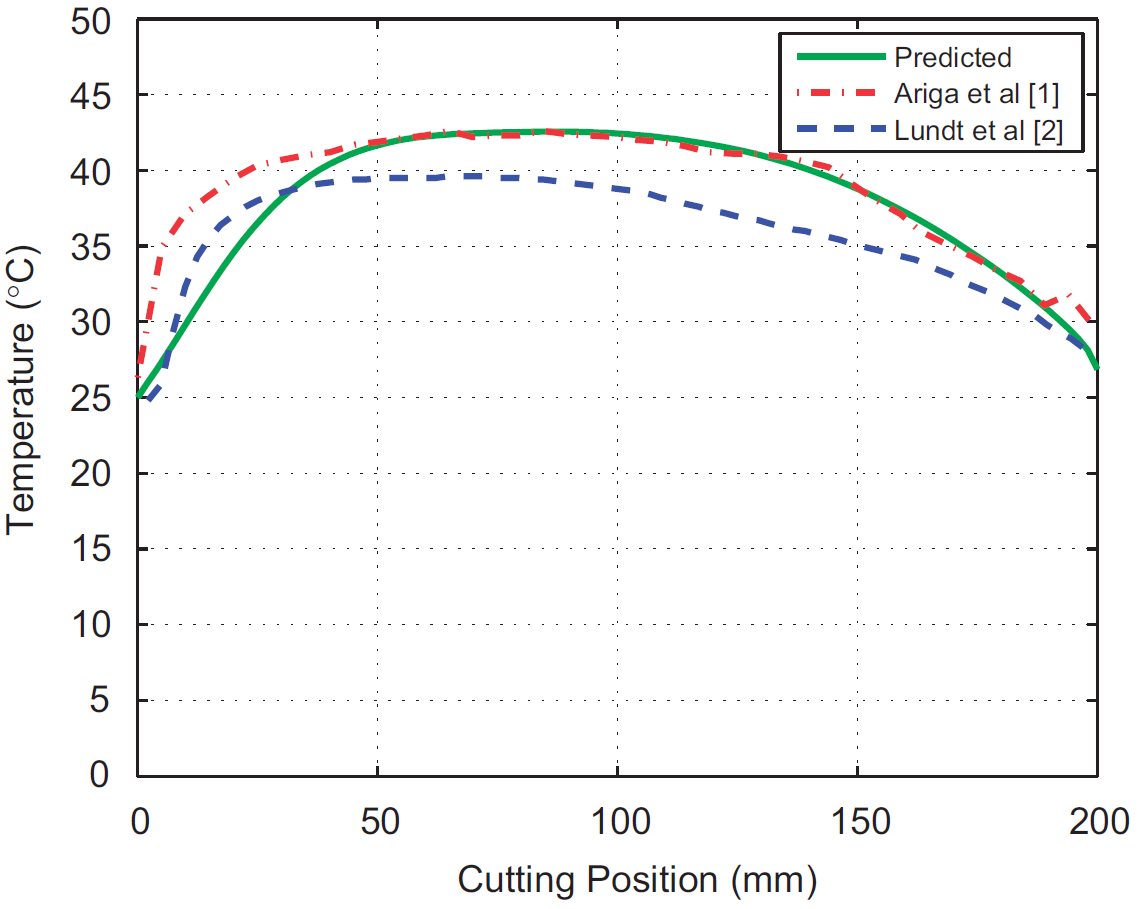
\includegraphics[width=4.0in]{temp-rise-bhagavat.PNG}
        \captionof{figure}{Temperature profile predicted by Bhagavat \& Kao during Wire Sawing}
        \label{fig:temp-rise}
 \end{minipage}

\subsubsection{Material Removal Rate}
Moller el al [ref] have developed several models to relate the material removal with cutting speed and wire load based on the indentation created by particles on the surface of the ingot. The amount of indentation was found out to be dependent mainly upon the frequency of abrasive particles touching Si surface per unit length. Material removal occurs by propagation of the cracks developed from indentation. They further distinguish the cutting process between a non-contact and a semi-contact regime based on the distance between the wire and the ingot surface with respect to the abrasives size. Semi-contact regime is predicted at high stress and low velocities and non-contact regime at low stress and high velocities.

The material removal rate $v_{s}$ as per their model can be written as:

\begin{equation}
v_{s} =  \frac{m \ \ V_{0}}{A_{s} \  \triangle t}
\label {cr-slip}
\end{equation}
\newline
Where, $m$ is the indentation events per unit contact area $A_{s}$ in time $\triangle t$ and $V_{0}$ is the material removed per indentation event. Based on indentation and fracture mechanics, $V_{0}$ has been found to be a function of normal force $F_{N}$ acting on the work piece as:
\begin{equation}
V_{0} = F^{2.2}_{N}
\label {cr-slip}
\end{equation}
\newline
As per these equations, it is clear that the material removal rate is a function of the contact length between the wire and the work piece since with increasing contact length, $A_{s}$ decreases. So for a cylindrical work piece, this result can be used for creating time steps depending upon the depth of cut while creating a numerical simulation for calculating the temperature and the stress fields during wire sawing.


%\subsection{Summary}
%In this chapter, theory of dislocation kinetics in silicon has been discussed first. Followed by this, works on numerical simulation of direction solidification based on the theory of dislocation kinetics has been discussed. Finally theory of wire sawing has been discussed. The various equations used are summarised below